\section{Test}\label{Test}
In this section, the testing, done on \lang{} to ensure the correctness of the output of the compiler, is described. 
\subsection{Compilation testing}
In order to keep track of whether or not something suddenly changed in the compiler implementation, both intentionally and unintentionally, a test was implemented to compare the current output of the compiler to a correct output of the compiler. This is based on a test file written in \lang{}, called \textit{BFGLtest.bfgl}. This makes sure that no unintentional changes happen, and that the compiler output stays the same. 
The comparison itself is done in several tests:
\begin{itemize}
    \item Test if the compilation \textit{out} folders are created.
    \item Test of the contents of the compilation \textit{out} folders, for example if they contain the right amount of files.
    \item MD5 comparison of all the files in the \textit{out} folders, to ensure that the files are all the exact same. 
\end{itemize}
The MD5 comparison uses a built-in class called "MessageDigest" from the java platform package "Security", which can produce MD5 hashes when given a binary representation of a data-object. The hashes of the objects are then compared. The implementation is as seen on figure \ref{fig:md5}.

\begin{figure}[H]
    \centering
    \begin{lstlisting}
        String hexCompiledFile;
        String hexTargetFile;
            if (targetFile != null && compiledFile != null){
                hexTargetFile = (new HexBinaryAdapter()).marshal(md5.digest(targetFile.getBytes()));
                hexCompiledFile =  (new HexBinaryAdapter()).marshal(md5.digest(compiledFile.getBytes()));

                if (hexTargetFile != null && hexCompiledFile != null){
                    assertTrue("Files are different! MD5 mismatch!" + i, hexTargetFile.equals(hexCompiledFile));
                }
            }
    \end{lstlisting}
    \caption{How the \lang{} compiler testing compares files using MD5.}\label{fig:md5}
\end{figure}

"assertTrue" is from the testing framework, and will report back whether or not the test failed. "MD5" is the MessageDigest object set to produce hashes.

The tests are build using Junit4, which is a testing framework that comes bundled with the IDE used in the development process(Intellij IDEA, \cite{intellij}). The use of Junit4 allows more time to be spent on the tests themselves, instead of spending a lot of time on the setup of the testing suite/program. It also allows to separate tests for different parts of the compiler into different classes, and then calling them all through a "Test Suite" that runs the tests. 
\todo{add intellij to bibtex breh}


\subsection{Blackbox tests}
This kind of test is not about programatically checking the code/compiler output for errors and unintended change. It is about running the compiler through extreme use-cases and other critical points to see if it still behaves accordingly, and visually verifying that this is the case. This was done throughout the implementation of the compiler, but in larger amounts during the codegen phase, as this was when the Test Suite was created. The following things were tested:
\begin{itemize}
    \item Evaluation order of functions.
    \item Behaviour on buffer overflow with Int datatype.
    \item If there are any illegal nested classes.
    \item Variables only allowed to exist in expressions.
    \item Only specific eventhandlers allowed, eg OnUpdate.
    \item Library import working.
    \item Jar output of compilation working.
\end{itemize}
This was all visually confirmed, as these are hard to confirm programmatically.

\subsection{Testing by doing}
Probably the most important test of them all is whether or not the language can actually be used to write games. To test this, a number of games were created in \lang{}, all of which were made to test different parts of the language. \todo{Dette modsiger det der staar i snake kinda :))}
Two of the games created was a classic Ping Pong game, and a Snake game.
\subsubsection{Ping Pong}
The Ping Pong game was used to test the maximum number of entities on the screen at once, as well as testing input methods and graphics. Up to a thousand entities on the screen at once slowed down the performance very significantly, but the game did not crash. This shows that the language, and the Slick libraries, are reliable enough for the purposes they were chosen for. The language can handle most of what a beginner would make in the language. The game running with 4 entities ran with no crashes, and no compiler related crashes or bugs appeared. A screenshot of the finished game can be seen on figure \ref{fig:pingpong}.
\begin{figure}[H]
    \centering
    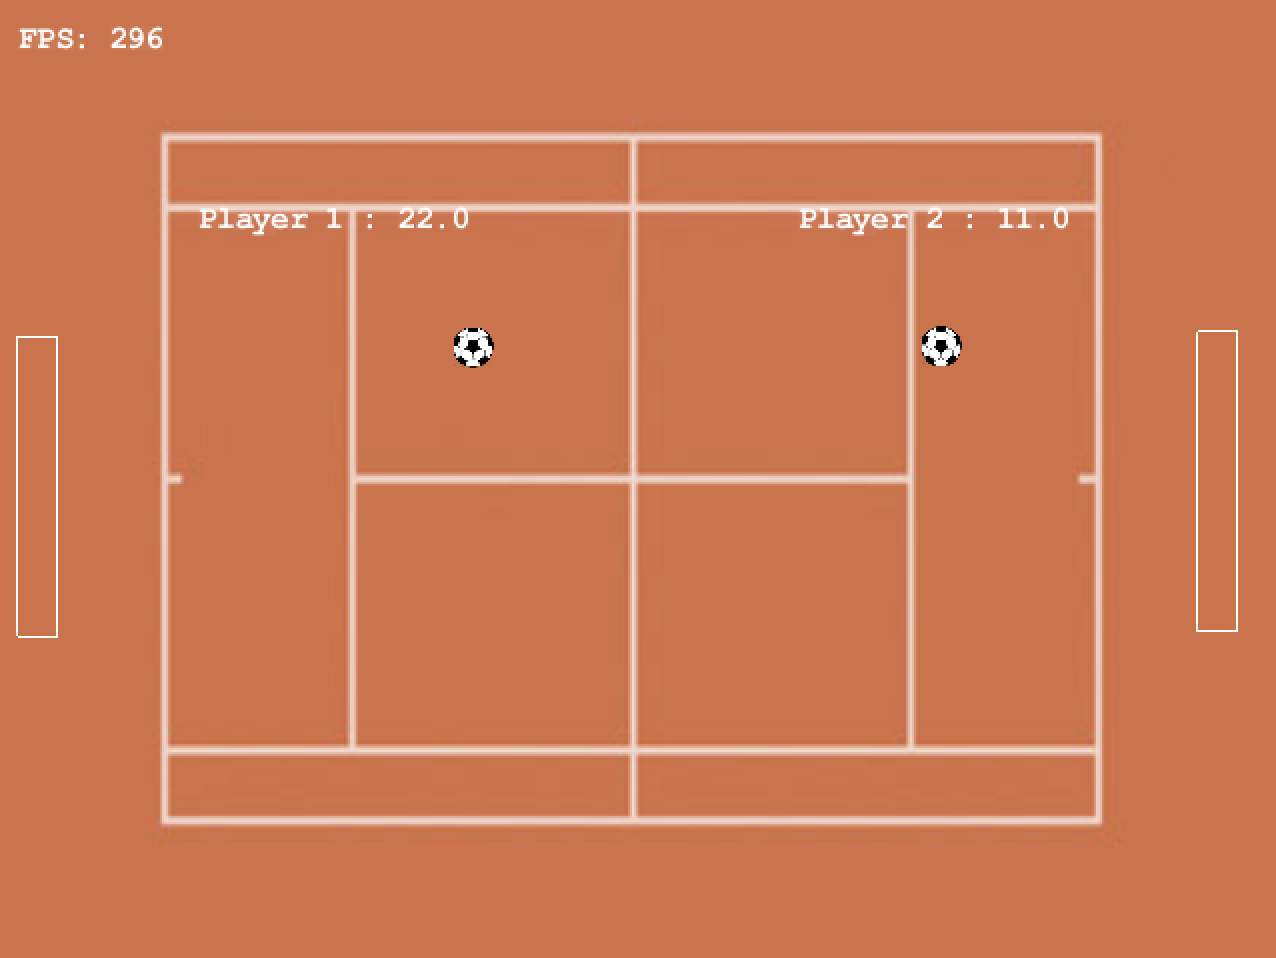
\includegraphics[scale=0.4]{resources/Images/newscreenshot.png}
    \caption{The Ping Pong game as it looked when used for testing.}\label{fig:pingpong}
\end{figure}

\subsubsection{Snake}
The Snake game was used to test the same things as Ping Pong was. Ping Pong was written in around 130 lines, and Snake in about 200 lines. The goal with writing Snake was not to test out different aspects of the language, different from the ones tested in Ping Pong, but to test out the writability of the language.
\pagebreak